%Correct the file name.
%X: book number
%Y: part number
%ZZZ: page number in three digits. So page 3 would be 003.

\documentclass[11pt]{amsbook}

\usepackage{../HBSuerDemir}	% ------------------------


\begin{document}
\setcounter{page}{310}
\setcounter{section}{4}
\setcounter{exercise}{62}
% =======================================================
\begin{exercise}
	Given
	% ++++++++++++++++++++++++++++++++++++++
	\hPage{b2p2/310}
	% ++++++++++++++++++++++++++++++++++++++
	\begin{equation*}
		z = \int_{0}^{x} e^{y^2} \cos{(x-y)}dy
	\end{equation*}
	find $ z_x.z_y$.
\end{exercise}

\begin{exercise}
	Same question for
	\begin{equation*}
		z = \int_{x}^{x^2} \ln{\arrowvert xy \arrowvert}dy
	\end{equation*}
\end{exercise}

\begin{exercise}
	Show that
	\begin{equation*}
		y = \frac{1}{k} \int_{0}^{x} f(\alpha) \sin{k(x-\alpha)} d\alpha
	\end{equation*}
	satisfies the relation
	\begin{equation*}
		\frac{d^2y}{dx^2} + k^2y = f(x).
	\end{equation*}
\end{exercise}
% =======================================================
\section*{ANSWERS TO EVEN NUMBERED EXERCISES}
\setcounter{exercise}{15}
\begin{exercise}
	$a) -2, \enskip b) 0$
\end{exercise}
\addtocounter{exercise}{5}
\begin{exercise}
	$0$
\end{exercise}
\addtocounter{exercise}{1}
\begin{exercise}
	$a) 0.17, \enskip b) 1.35$
\end{exercise}
\addtocounter{exercise}{1}
\begin{exercise}
	$74.0 m^2$
\end{exercise}
\addtocounter{exercise}{1}
\begin{exercise}
	$a) -Sech\,2t, \enskip b) (\frac{1}{t^2} \cos{\frac{t-1}{t}} + 2t\sin{\frac{t-1}{t}}) e^{t^2}$
\end{exercise}
\addtocounter{exercise}{3}
\begin{exercise}
	$-\frac{3y+1}{3x+1}$
\end{exercise}
\addtocounter{exercise}{5}
\begin{exercise}
	$12u^2 - 24uv -12v^2$
\end{exercise}
\addtocounter{exercise}{7}
\begin{exercise}
	on $\Gamma : 4x-2y=3, \enskip z=x^2-y^2$
\end{exercise}
\addtocounter{exercise}{1}
\begin{exercise}
	$a) (1,2,0), \enskip b) (\alpha, \beta, \gamma)$
\end{exercise}
\addtocounter{exercise}{1}
\begin{exercise}
	$a) \frac{-20}{\sqrt{17}}, \enskip b) (\frac{\pi}{\sqrt{3}} - \ln{4}) / \sqrt{4 + \pi^2}$
\end{exercise}
\addtocounter{exercise}{1}
\begin{exercise}
	$a) (-3e^2\cos{1}-e^2\sin{1}+2e)/\sqrt{14}, \enskip b) \frac{5}{26}$
\end{exercise}
\addtocounter{exercise}{1}
\begin{exercise}
	$a) (-12e^2 + 5e - 5)/7, \enskip b) \frac{2}{\sqrt{6}}$
\end{exercise}
% =======================================================
\end{document}  

%==== templates ====

%==== environments ====

%\begin{figure}[htb]
%	\centering
%	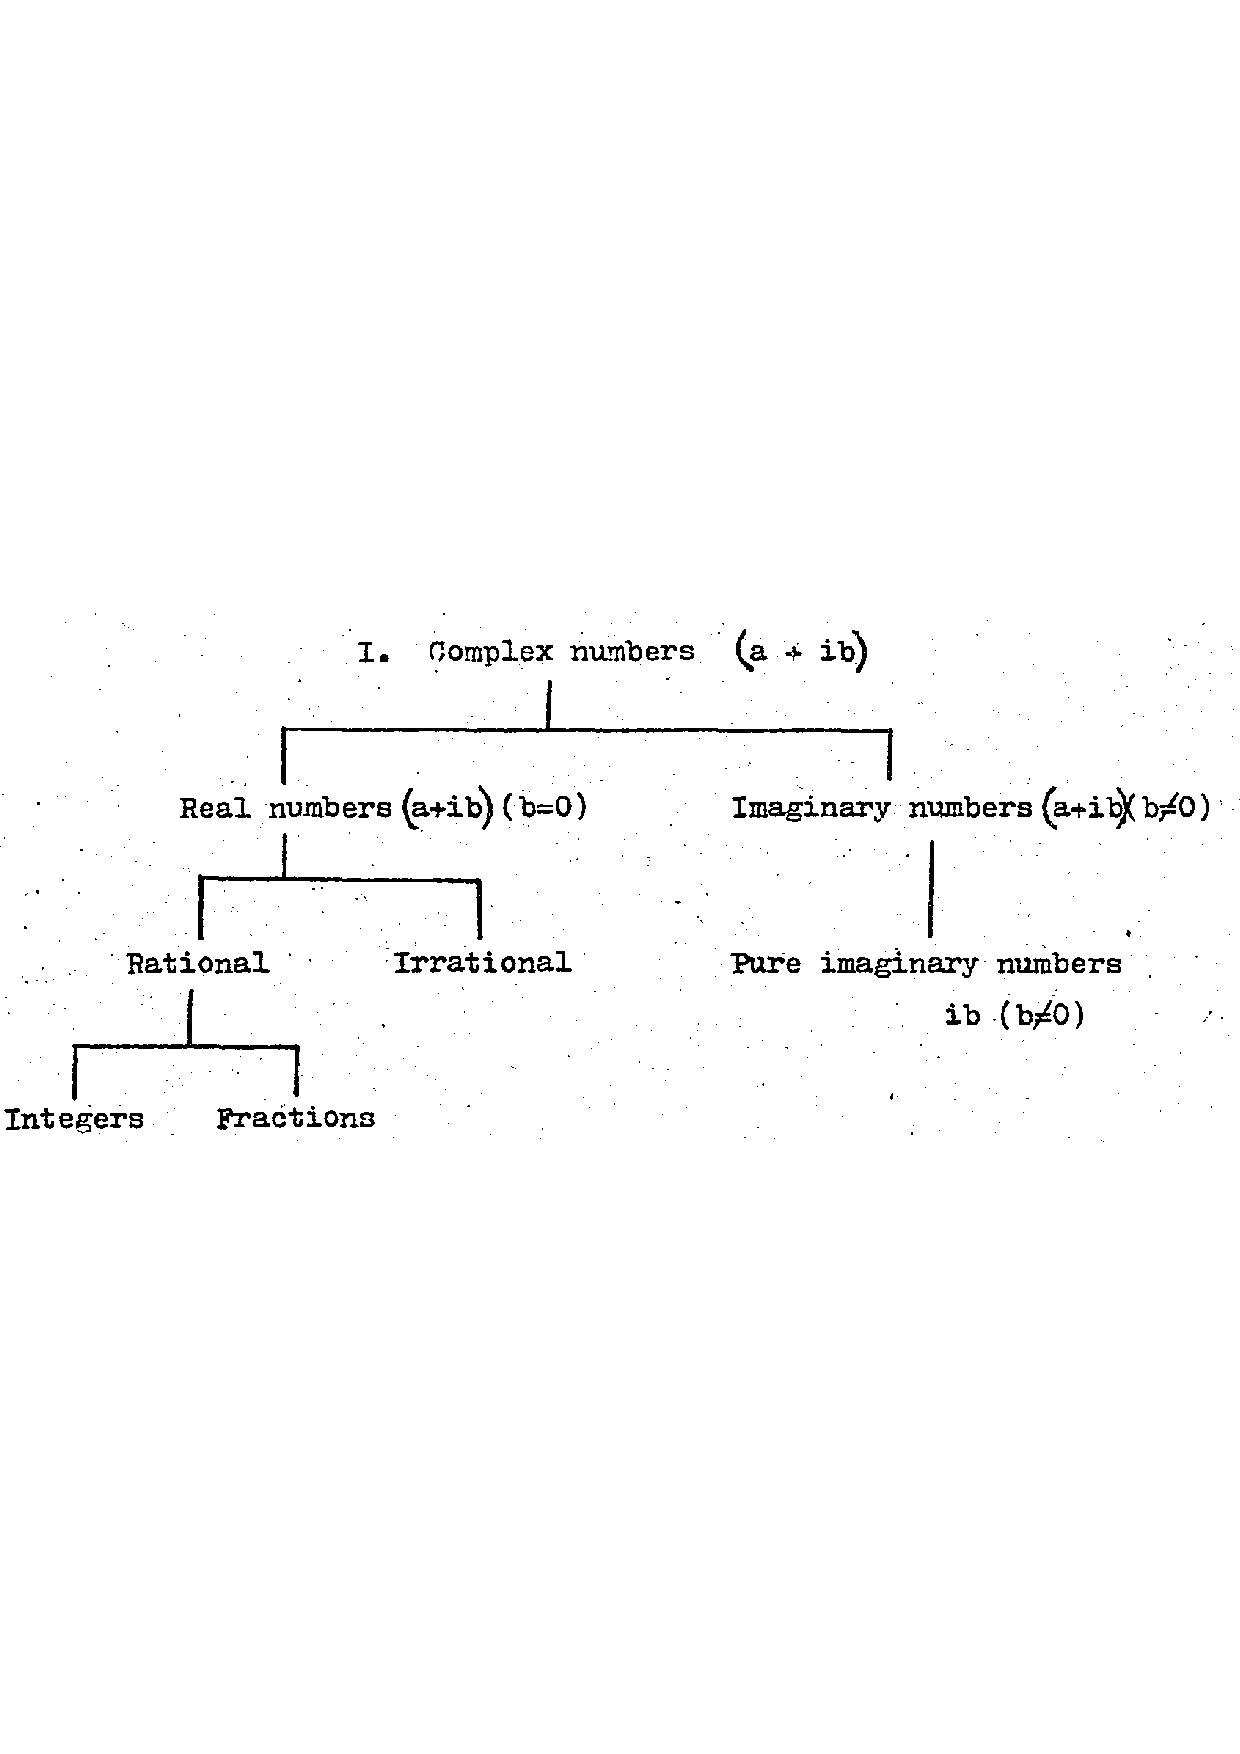
\includegraphics[width=0.9\textwidth]{images/SD-1-1p15A}
%	\caption{Classification of complex numbers}
%	\label{fig:classificationOfComplexNumbersA}
%\end{figure}

%\begin{center}
%\begin{tabular}{cc}
%\end{tabular}
%\end{center}

%\begin{exmp}
%\begin{hSolution}
%\end{hSolution}
%\end{exmp}

%\begin{hEnumerateAlpha}
%\end{hEnumerateAlpha}

%\begin{hEnumerateRoman}
%\end{hEnumerateRoman}

%$
%\begin{bmatrix}
%\end{bmatrix}
%$

%\frac{aaaa}{bbb}
%\frac{a_{n}}{b_{n}}
%\left( aaaa \right)
%\Longrightarrow

%\begin{multicols}{2}
%	bb
%\columnbreak
%	aa
%\end{multicols}
